\chapter{Implementierung}\label{chapter:implementierung}
Die Anwendung besteht grundlegend aus einer \textit{\nameref{class:mainactivity}} in welche die verschiedenen Fragments geladen werden.\\
Jedes Fragment wurde dabei nach dem in Android üblichen Pattern für Fragments entwickelt, welches aus einem \textit{Fragment}, das für die optische Darstellung der Informationen zuständig ist, und einen \textit{ViewModel}, welches die Daten verarbeitet und an das Fragment übergibt, implementiert.\\
Im folgenden werden die implementierten Klassen und Konzepte der entwickelten Anwendung einmal genauer betrachtet.

\section{MainActivity}\label{class:mainactivity}
Die \textit{MainActivity} wird ausgeführt sobald die Anwendung vom Nutzer gestartet wird.\\
In dieser Klasse wird der Hauptbildschirm erzeugt, der aus einem \textit{Hostfragment}, in welches dann später die einzelnen Fragments geladen werden, und der \textit{BottomNavigationView} besteht. \\
Um der Navigationsleiste ein Funktion zuzuweisen, muss in der \textit{onCreate}-Methode der \textit{NavController} erstellt werden. Dieser steuert die einzelnen Buttons der \textit{BottomNavigationView} und lädt die zugehörigen Fragments in das \textit{Hostfragment}. Über diese Leiste stehen dem Nutzer auf die Ansichten \nameref{impl:ar}, \nameref{impl:verwaltung} und \nameref{impl:generator} zur Verfügung.


\section{Augmented Reality}\label{impl:ar}
Die wichtigste Ansicht der Anwendung stellt die AR-Funktion dar. \\ 
Sie zeigt dem Nutzer das Kamerabild und fügt die 3D-Modelle in dieses ein.\\
Diese Ansicht wird durch das \textit{ARCameraFragment} bereitgestellt.
Die Struktur, die zur Umsetzung der Augmented Reality genutzt wurde, beruht zum Großteil auf dem Konzepten und Klassen von ARToolKit und wurde dann an die Anforderungen dieser Arbeit angepasst.

\subsection{ARCameraFragment}
Das \textit{ARCameraFragment} bildet den Grundbaustein des Augmented Reality Fragments und erweitert das \textit{ARFragment}.
Es erzeugt die visuelle Oberfläche in Form eines \textit{FrameLayouts}, welches ein \textit{GLSurfaceView} enthält, auf dem später das Kamerabild, sowie die Modelle projiziert werden. \\
Des weiteren überschreibt die Klasse die abstrakten Methoden des \textit{ARFragments} und weist diesem  einen \textit{ARRenderer} und das \textit{FrameLayout} zu.

\subsection{EducationARRenderer}
Die \textit{EducationARRenderer}-Klasse erweitert ARToolKits \textit{ARRender}. Die Aufgabe des Renderes ist es die AR-Szene zu konfigurieren und die Visualisierung der AR-Modelle einzuleiten. \\
Dazu werden zunächst alle Modelle geladen und die Instanzen der \textit{Modell}-Klasse in einer ersten Hashmap gespeichert. Des weiteren werden die folgenden Klassen der \textit{ARRenderer}-Klasse überschrieben.

\subsubsection{configureARScene()}
In dieser Klasse wird die AR-Szene konfiguriert. Dazu wird zunächst für jedes Modell der Marker mit der zugehörigen ID erzeugt und die sogenannte UID, die zurückgeliefert wird und auf den Marker verweist, zusammen mit dem Modell in einer zweiten Hashmap gespeichert.

\subsubsection{draw()}
Diese Methode dient dazu die \textit{draw}-Funktion der \textit{Modell}-Klassen aufzurufen, wenn der Marker des Modells im Kamerabild gefunden wurde.\\
Dafür durchläuft die Methode mit Hilf der UIDs alle Marker und generiert die Model-, View- und Projektionsmatrizen der gefundenen Marker. Diese Matrizen werden dann an die entsprechenden \textit{draw}-Methoden der Modelle weitergegeben, um die Modelle in der richtigen Transformation zu visualisieren. 


\section{Modellverwaltung}\label{impl:verwaltung}
Eine der drei Hauptfunktionen der Anwendung stellt Modellverwaltung dar. Diese besteht eigentlich zwei einzelnen Fragments, dem \textit{AdministrationFragment} und einem weiterführenden Fragment, dem \textit{UploadFragment}. Das \textit{AdministrationFragment} wird geladen, sobald der Nutzer in der Navigation die Modellverwaltung aufruft. Hier kann der Nutzer eine Liste mit seinen hoch geladenen Modellen betrachten, und diese gegebenenfalls löschen. \\
Über einen Plus-Button wird ein Nutzer auf das \textit{UploadFragment} weitergeleitet. Dieses erlaubt es dem Nutzer Modelle aus den Dateien hochzuladen. 

\subsection{AdministrationFragment}
Wie bereits beschrieben ist es die Aufgabe dieser beiden Klassen die Modelle des Nutzers zu Verwalten und wird aufgerufen sobald der Nutzer über die Navigation die Verwaltung auswählt. \\
Dafür wird dem Nutzer über das \textit{AdministrationFragment} eine graphische Oberfläche bereit gestellt. Dafür werden über die \textit{ModelManager}-Klasse alle Modelle des Nutzers eingeholt und für jedes Modell über die \textit{createNewElem()}-Methode eine Zeile im Layout in Form eines horizontalen linearen Layouts erstellt.\\
Des weiteren wird ein Button erzeugt, welcher über einen \textit{OnClickListener} das \textit{UploadFragment} aufruft.

\subsubsection{createNewElem()}
Diese Methode erzeugt die graphische Darstellung eines Modelles im \textit{AdministrationFragment}.\\
Dazu wird auf Grundlage der übergebenen Parameter eine horizontales lineares Layout erstellt, welches beginnt mit einem Switch-Button, der zunächst nicht implementiert wurde, aber später dazu genutzt werden soll ein Modell zu aktivieren oder zu deaktivieren. Anschließend folgt die eindeutige MarkerID des Modelles und der Name. Zuletzt folgt ein Button zum Löschen des Markers, der über einen \textit{OnClickListener} die \textit{deleteModel()}-Methode der \textit{ModelManager}-Klasse aufruft.

\subsection{UploadFragment}
Dieses Fragment wird über den Hinzufügen-Button der \textit{AdministrationFragment}-Klasse aufgerufen und erzeugt dem Nutzer eine graphische Oberfläche zum hochladen von Modellen. \\
Dazu werden dem Nutzer verschiedene Eingabefelder zur Verfügung gestellt.\\
Das erste ist ein Texteingabefeld, über welches dem Modell ein Name zugeordnet wird. Initial wird dieses Feld mit dem Namen \glqq Modell-\textit{MarkerID}\grqq erzeugt.\\
Anschließend folgen zwei Buttons zum Auswählen der Texturdatei und der Modelldatei. Über einen \textit{OnClickListener} wird ein \textit{Action Open Document}-Intent erzeugt, sobald der Button gedrückt wird. Dieser Intent erzeugt ein Dialog zur Dateiauswahl, über den der Nutzer auf seinen lokalen Speicher, sowie GoogleDrive, zugreifen kann. Das Ergebnis des Intents kann dann über die Callback-Methode \textit{onActivityResult()} abgerufen werden. \\
Des weiteren wird ein Button zum Hinzufügen des Modells bereitgestellt, welcher die Methode \textit{addModel()} der \textit{UploadViewModel}-Klasse aufruft.

\subsubsection{onActivityResult()}
Bei dieser Methode handelt es sich um eine Callback-Methode, die die Ergebnisse eines Intents abruft.\\
Dazu wird anhand eines Codes geprüft, um was für eine Rückgabe es sich bei den empfangen Daten handelt und ob das Ergebnis erfolgreich war. 
Anschließend wird dann, falls es sich bei der Rückgabe um den gewählten Dateipfad zu einer der Modelldateien handelt, der entsprechende Pfad an das \textit{UploadViewModel} übergeben.

\subsection{UploadViewModel}
Das \textit{UploadViewModel} stellt die Daten für das \textit{UploadFragment} zur Verfügung. Dazu wird das Konzept der \textit{MutableLiveData} genutzt, welche vom \textit{UploadFragment} über einen \textit{Observer} beobachtet werden können. Diese werden im Viewmodel initial erzeugt und werden dann über Nutzereingaben vom \textit{UploadFragment} aktualisiert. Lediglich die MarkerId wird anfänglich generiert und im Anschluss nicht mehr verändert. Dazu wird die \textit{getNextID()}-Methode der \textit{ModelManager}-Klasse aufgerufen. Diese liefert dem \textit{UploadViewModel} die nächste freie ID zurück.

\subsubsection{addModel()}
Diese Methode wird vom \textit{UploadFragment} aufgerufen und fügt das Modell zu den Modellen des Nutzers hinzu, falls alle benötigten Daten vom Nutzer angegeben wurden.\\
Ist dies der Fall werden die Modell über die \textit{transferToInternalStorage()}-Methode der \textit{FileManager}-Klasse in den internen Speicher der Anwendung kopiert. Des weiteren wird über die Methode \textit{addModel()} der \textbf{ModelManager}-Klasse eine Referenz auf die Dateien abgespeichert. \\
Anschließend wird der Nutzer auf das \textit{ConfirmationFragment} weitergeleitet.

\subsubsection{requierdDataAvailable()}
Diese Methode prüft, ob der Nutzer alle Daten angegeben hat, die benötigt werden, um das Modell hochzuladen.

\subsubsection{correctFileType()}
Diese Methode wird dazu genutzt, um zu überprüfen, ob es sich bei der Modelldatei, die der Nutzer wählt, um eine Obj-Datei handelt. Dazu wird der Dateiname der Modelldatei abgefragt und die Endung der Datei geprüft. Eine solche Überprüfung ist bei der Texturdatei nicht nötig, da an dieser Stelle über den MIME-Type, die Auswahl eingeschränkt werden kann.

\subsection{ConfirmationFragment}
Das \textit{ConfirmationFragment} wird aufgerufen wenn der Nutzer ein Modell hochgeladen hat. Dabei wird die MarkerID des Modells und dessen Name an das Fragment übergeben. Mit Hilfe der ID generiert das Fragment über die \textit{generateMarker()}-Methode der \textit{MarkerGenerator}-Klasse den Marker der zum Modell gehört und zeigt diesen in einem \textit{ImageView} an.\\
Über einen Button hat der Nutzer die Möglichkeit den Marker abzuspeichern. Per \textit{OnClickListener} wird ein \textit{Intent} erzeugt der dem Nutzer einen Dialog öffnet in dem er einen Ordner zum Abspeichern des Markers auswählen kann. 

\subsubsection{onActivityResult()}
Diese Methode stellt die Callback-Methode zur Behandlung von \textit{Intents} dar. Hier wird die \textit{saveBitmap()}-Methode der \textit{Filemanager}-Klasse aufgerufen, nachdem der Nutzer einen Dateipfad zum Abspeichern des Markers gewählt hat.


\section{Markergenerierung}\label{impl:generator}
Diese Funktion stellt die letzte Ansicht dar, die über die Navigationsleiste aufgerufen werden kann.\\
Sie besteht lediglich aus dem \textit{MarkerFragment}, mit dessen Hilfe der Nutzer einen Marker, den er zum Beispiel gelöscht hat, erneut generieren kann.

\subsection{MarkerFragment}
Das \textit{MarkerFragment} stellt dem Nutzer eine Oberfläche mit einem Eingabefeld und einem Button zur Verfügung.\\
In das Eingabefeld kann der Nutzer, die ID eines Modelles, welche er aus der Modellverwaltung entnehmen kann, eintragen. Drückt dieser anschließend den Button, wird über einen \textit{OnClickListener} der zugehörige Marker zu der ID mit der \textit{generateMarker}-Methode der \textit{MarkerGenerator}-Klasse aufgerufen und die zurückgelieferte Bitmap des Markers in einem \textit{ImageView} angezeigt. \\
Des weiteren wird ein Button zum Speichern des Markers mit den analogen Funktion des Buttons im \textit{ConfirmationFragments} zur angezeigt.


\section{Shader Implementierung}
Zum Rendern der Modelle mussten die folgenden eigene Shader implementiert werden. Diese beruhen im Grundgerüst auf den von ARToolkit bereitgestellten Beispielimplementierungen der Shader und wurden um die Anforderungen dieser Arbeit erweitert. So wurde beispielsweise eine Unterstützung von Texturen implementiert.

\subsection{MyShaderProgram}
Die Klasse \textit{MyShaderProgram} erweitert ARToolKits Klasse \textit{ShaderProgram}. \\
Die wichtigste Eigenschaft dieser Klasse ist es, dass sie die \textit{render()}-Methode der \textit{ShaderProgramm}-Klasse überschreibt.

\subsubsection{render()}
Diese Methode wird aufgerufen um ein Modell zu rendern. \\
Dazu werden zunächst die Verticies, Farbinformationen, Normalenvektoren und Texturkoordinaten an OpenGL übergeben. \\
Im letzten Schritt wird dann das Modell aus vielen einzelnen Dreiecken mit OpenGLs \textit{drawArrays()}-Funktion gezeichnet.

\subsection{MyVertexShader}
Damit OpenGL den Shader ausführen kann muss dieser in der Programmiersprache OpenGL Shading Language (GLSL) geschrieben sein. \\
Der String \textit{vertexShader} enthält diesen in GLSL geschriebenen Shader.

\subsection{Vertex Shader}
In dem Shader selbst wird der finale Punkt von jedem Vertex aus der \textit{Projection}-Matrix, der \textit{ModelView}-Matrix und dem ursprünglichen Vertexvektor berechnet. Dieser wird dann zusammen mit der Farbe, der Texturkoordinate und des Noramlenvektors an den Fragment Shader, der in der Klasse \textit{MyFragmentShader} i9mplementiert wird, weitergeleitet.

\subsubsection{configureShader()}
Diese Methode konfiguriert einen Shader und übergibt den String mit dem Vertex Shader an OpenGL.


\subsection{MyFragmentShader}
Auch dieser Shader muss über den String \textit{fragmentShader} in GLSL implementiert werden.

\subsubsection{Fragment Shader}
In dem Shader, der über den String definiert wird, wird die Farbe für jedes Fragment aus der vom Vertex Shader übergeben Farbe, und übergebenen Textur berechnet. 

\subsubsection{configureShader()}
Diese Methode konfiguriert einen Shader und übergibt den String mit dem Fragment Shader an OpenGL.



\section{Hilfsklassen}
Im Folgenden werden ein paar Hilfsklassen vorgestellt, die genutzt wurden, um den Restlichen Klassen wichtige Funktionen zur Verfügung zustellen.

\subsection{FileManager}
Der \textit{FileManager} dient dem Zweck alle Funktionen bereitzustellen, die benötigt werden um die Dateien zu verwalten, die die Anwendung benötigt.

\subsubsection{saveBitmap()}
Die \textit{saveBitmap()} Methode speichert ein Bild, welches in Form einer Bitmap übergeben wird, an einem bestimmten Dateipfad, der über die Methodenparameter übergeben wird. \\
Dazu wird ein \textit{OutputStream} erzeugt auf welchen die Datei dann in Form einer jpeg-Datei geschrieben wird.

\subsubsection{transferToInternalStorage()}
Diese Methode kopiert eine Datei von einem Ort in den internen Speicher. Dazu wird ein \textit{InputStream} zum lesen der Datei und ein \textit{OutputStream} zum schreiben der Datei geöffnet. Anschließend wird die Datei Stück für Stück eingelesen und auf den \textit{OutputStream} geschrieben.

\subsubsection{printInternalStorage()}
Dieses ist eine Hilfsmethode zum ausgeben des internen Speichers. Sie wurden zum Debuggen verwendet.


\subsection{MarkerGenerator}
Der \textit{MarkerGenerator} ist eine Hilfsklasse, die dazu zuständig ist einen Marker mit einer bestimmten ID zu generieren, der dann von den AR-Klassen getrackt werden kann.\\ Die Hauptfunktion ist dabei die Methode \textit{generateMarker()}.

\begin{figure}
\centering
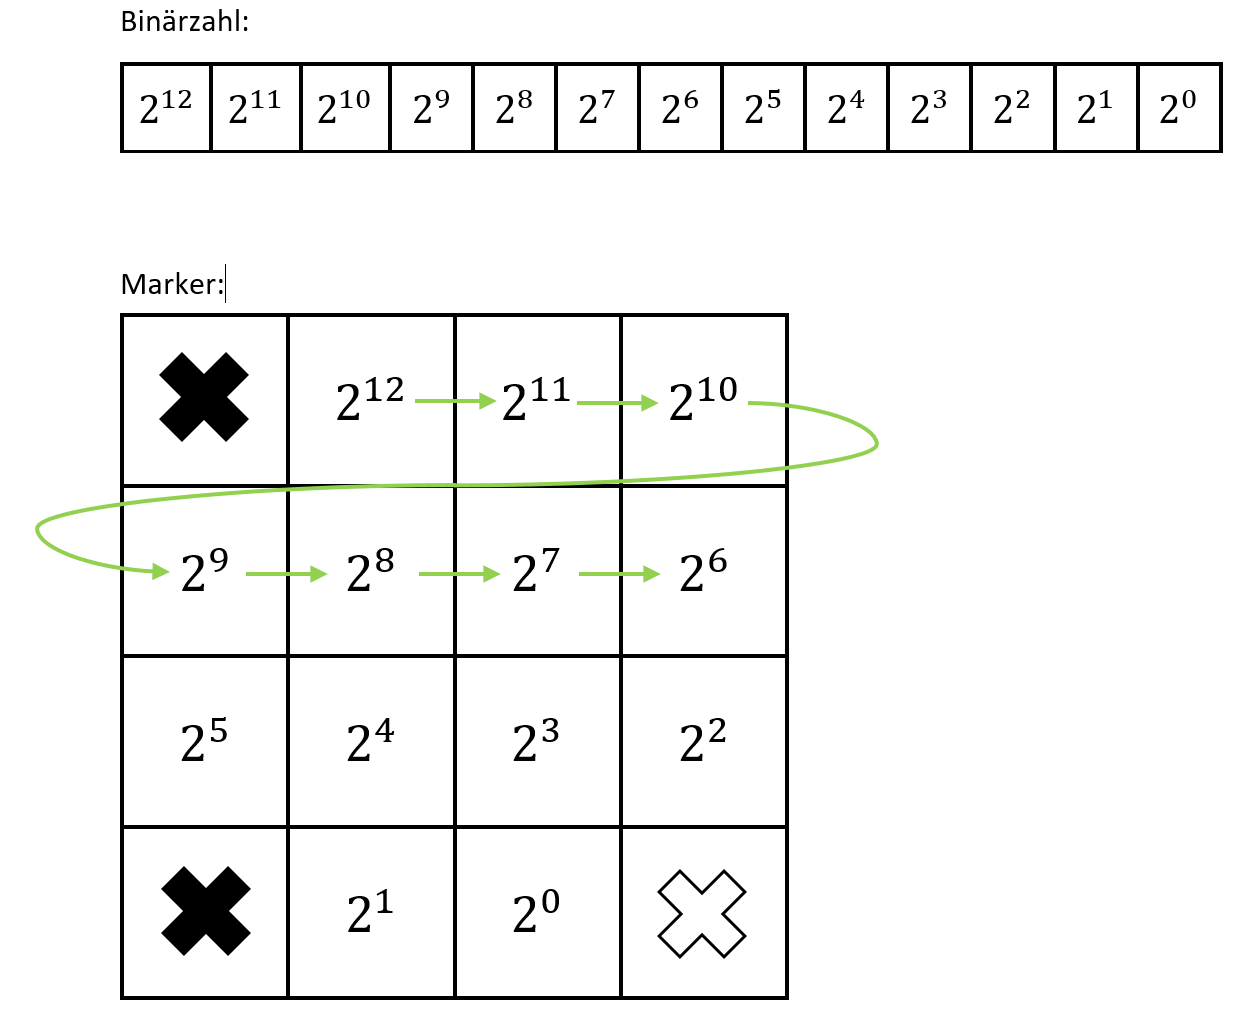
\includegraphics[width=0.8\textwidth]{Abbildungen/barcode-creation.png}
\caption[Markererstellung]{Visualiserung des Vorgehens zur Erstellung eines 4x4 Barcodepatterns. (Quelle: Eigene Darstellung)}
\label{fig:barcode-creation}
\end{figure}

\subsubsection{generateMarker()}
Die \textit{generateMarker}-Methode erzeugt einen Marker mit einer bestimmten ID und Patterngröße $n$, die über die Methodenparameter übergeben werdem. Dazu wird zunächst eine quadratische Bitmap der Größe $n$ x $n$ erzeugt. Anschließend muss aus der übergebenen ID ein Barcodemuster erzeugt werden.
Dazu muss die ID mit der \textit{getCodedID()}-Methode in eine kodierte Binärzahl in Form eines Strings umgewandelt werden.\\
Im nächsten Schritt kann dann die Bitmap Feld für Feld durchlaufen werden und der Wert des Strings an der Stelle $i*n + j$ eingefügt werden, wobei $i$ die aktuelle Zeile und $j$ die die aktuelle Spalte repräsentiert. \\ 
In einem letzen Schritt wird die Grafik dann hochskaliert, damit sie besser in Dokumente eingefügt werden kann, und ein schwarzer Rahmen mit Hilfe der \textit{addBorder}-Methode um das Barcodepattern gezogen werden, um die Anforderungen von ARToolKit zu befriedigen.

\subsubsection{getCodedID()}
Diese Methode erzeugt aus einer ID einen kodierten String der das Pattern des Barcodemarkers repäsentiert. 
Dieses geschieht indem die ID zunächst in eine Binärzahl mit der Länge $n^2 - 3$ umgewandelt wird. Jede Null in der Binärzahl repräsentiert ein weißes Feld und jede Eins ein schwarzes Feld im Barcodepattern. Damit das Pattern am Ende jedoch Rotationsinvariant ist sind insgesamt drei Felder des Musters bereits eine feste Farbe zugeordnet(in Abbildung \ref{fig:barcode-creation} durch Kreuze in der entsprechenden Farbe dargestellt). Für diese vordefinierten Felder werden deshalb entweder eine Null oder eine Eins an den entsprechenden Stellen des Strings, der die Binärzahl repräsentiert , eingefügt.


\subsection{Model}\label{class:model}
Diese Klasse repräsentiert ein Modell, welches vom Nutzer hochgeladen werden kann. Dabei speichert je eine Instanz der Klasse die für das Rendering relevanten Informationen von je einem Modell. \\
Die \textit{Model}-Klasse beruht auf dem Grundgerüst von der \textit{Cube}-Klasse, welche ein Teil von ARToolKit ist und einen simplen Würfel darstellt.\\
Diese Klasse wurde im Rahmen der Arbeit so modifiziert, dass sie beliebige Modelle speichern kann.\\
Dazu werden mittels der \textit{\nameref{class:objloader}}-Klasse die Daten aus der Obj-Datei geladen und in Buffern gespeichert. Des weiteren wird mit Hilfe der \nameref{class:textureloader}-Klasse die Textur geladen und eine Referenz auf diese erzeugt.\\

\subsection{draw()}
Die \textit{draw}-Methode ist dafür zuständig das Modell zu rendern, in dem die Daten des Modells, sowie die Model-, View- und Projektionsmatrix des Markers, an eine Instanz der \textit{ShaderProgram}-Klasse des Modells übergeben werden.


\subsection{ObjLoader}\label{class:objloader}
Die \textit{ObjLoader}-Klasse ist dafür zuständig die Daten aus der Obj-Datei des Modells, welches der Nutzer hochgeladen hat, einzulesen und in das passende Format für OpenGL umzuwandeln.\\ 
Das Ganze geschieht über den Konstruktor \ref{method:objloader}, der die Daten ausließt und als Klassenvariablen des ObjLoaders speichert, sodass diese aus anderen Klassen abgefragt werden können.

\subsubsection{ObjLoader()}\label{method:objloader}
Der Konstruktor der Klasse bekommt über einen Parameter den Pfad zur Obj-Datei übergeben. \\
Nachdem diese geladen wurde, muss die Datei Zeile für Zeile durchlaufen werden und anhand der Abkürzungen, mit denen jede Zeile beginnt, der Datentyp bestimmt werden. \\
Der Aufbau einer Obj-Datei unterliegt dabei dem folgenden Muster (vergleiche dazu auch Abbildung \ref{fig:obj-datei}):\\
Jede Zeile enthält ein Datenobjekt, welches über die die Kennung zu einem bestimmten Datentyp zugeordnet werden kann. 
Zu Beginn der Datei werden alle Einzelteile des Modells definiert:
\begin{description}
\item[Vertex (v):] Ein Vertex repräsentiert einen Eckpunkt des Objektes. Dazu werden in der Zeile die drei Koordinaten des Punktes gespeichert.
\item[Textur (vt):] Diese Zeile besteht aus zwei Koordinaten, welche einen Punkt in einem zweidimensionalen Bild, der Texturdatei, repräsentieren.
\item[Normalenvektor (vn):] Dieser Kennung folgenden die drei Koordinaten eines Normalenvektors  
\end{description}
\begin{figure}
\centering
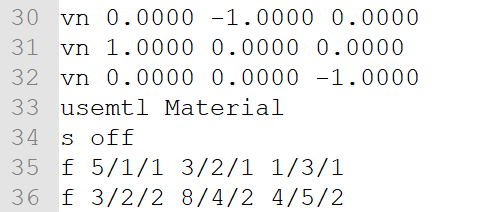
\includegraphics[width=0.6\textwidth]{Abbildungen/obj-datei.png}
\caption[Obj-Dateiformat]{Ausschnitt aus einer Obj-Datei. (Quelle: Eigene Darstellung)}
\label{fig:obj-datei}
\end{figure}
Damit OpenGL mit diesen Einzelteilen arbeiten kann, müssen diese noch zusammengesetzt werden. \\
Die dafür nötigen Informationen speichern die sogenannten Faces (deutsch: \glqq Gesichter\grqq ), welche die Kennung f besitzen. Sie beschreiben die einzelnen Flächen des Modells. Da zuvor im \nameref{chapter:Entwurf}) die Anforderung an die Obj-Dateien gestellt wurde, dass diese tranguliert werden, handelt es sich bei den Flächen immer um Dreiecke. \\ 
Die Zeile eines dieser Dreiecke speichert dafür für jeden Eckpunkt der Fläche drei Indices die auf jeweils einen der  zuvor definierten Vertices, Texturkordinaten und Normalenvektoren verweisen. Dadurch wird neben der Koordinaten der Fläche, auch der zugehörige Ausschnitt der Textur und der Normalenvektor der Datei definiert. \\
Das Programm erstellt aus diesen Daten drei Listen (jeweils eine für Vertices, Texturkoordinaten und Normalenvektoren), indem es für jede Fläche die Daten jedes Punktes an die entsprechende Liste anhängt.\\
Auf diese Listen kann dann über die Klassenvariablen des \textit{ObjLoader}-Objektes zugegriffen werden.

\subsection{TextureLoader}\label{class:textureloader}
Die \textit{TextureLoader}-Klasse hat die Aufgabe die Textur-Datei einzulesen und OpenGL zur Verfügung zu Stellen. Dazu wird zunächst mit \textit{GLES20.glGenTextures} eine Textur erzeugt und eine Referenz in \textit{textureHandle} gespeichert. Anschließend wird die Texturdatei des Modells als Bitmap an die Textur gebunden und die Filter zur Texturverarbeitung gesetzt. 

\section{ARToolKit-Klassen}
Dieses Kapitel deckt die wichtigsten Klassen, die zur Umsetzung der Augmented Reality genutzt wurden ab. Diese Klassen wurden im Laufe der Arbeit an vielen Stellen angepasst oder erweitert, um die Anforderungen der Arbeit zu erfüllen.

\subsection{ARController}
Der \textit{ArController} ist ein \textit{Singelton} der ARToolKit-Bibliothek, welcher den Zugriff auf die nativen Funktionen, die in der \textit{ARX\_jni}-Klasse definiert werden, regelt. \\

\subsection{ARX\_jni}
Die \textit{ARX\_jni}-Klasse enthält die \textit{Java Native Interface}-Funktionen und stellt die Schnittstelle zur Nativen ARToolKit Bibliothek dar. Diese Bibliothek enthält alle grundlegenden Funktionen von ARToolKit in C++ geschrieben.

\subsection{ARFragment}
Die \textit{ARFragment}-Klasse wurde im Laufe der Arbeit implementiert und ist von ihrer Funktionalität identisch zu der \textit{ARActivity}-Klasse von ARToolKit. Sie wurde lediglich an die Anforderungen eines Fragments angepasst, um in das Userinterface der Anwendung eingefügt werden zu können.\\ 
Bei ihr handelt es sich um eine Abstrakte Klasse, die das Grundgerüst des Fragments bildet, dass die AR-Inhalte anzeigen soll.\\
Die Hauptfunktionalität dieser Klasse ist es die graphische Oberfläche für die AR-Anwendung zu erzeugen. Dazu erzeugt die Klasse ein \textit{GLSurfaceView} und weist diesem einen Renderer zu, der später dazu zuständig ist die Modelle auf dem \textit{GLSurfaceView} anzuzeigen.\\
Des weiteren wird der Kamerastream geöffnet und dem \textit{GLSurfaceView} zugewiesen.

\subsubsection{supplyRenderer()}
Mit Hilfe dieser Methode wird der Klasse ein \textit{ARRenderer} übergeben. Diese Methode muss von der Klasse, die von dem \textit{ARFragment} erbt überschrieben werden, um den \textit{ARRenderer} zusetzen.

\subsubsection{supplyFrameLayout()}
Diese abstrakte Methode übergibt das \textit{FrameLayout} auf dem die Augmented Reality erzeugt werden soll an die \textit{ARFragment}-Klasse. Dazu muss diese Methode von der Erbenden Klasse überschrieben werden.

\subsection{ARRenderer}
Der \textit{ARRenderer} ist eine abstrakte Klasse aus der ARToolKit-Bibliothek und bildet das Grundgerüst für den Renderer, welcher in einer Anwendung die ARToolKit nutzt implementiert werden muss.\\
Dazu wird unter anderem das Rendern des Videohintergrunds initialisiert.

\subsection{ShaderProgram}
Diese abstrakte Klasse bildet das Grundgerüst eines Shader Programms. \\
Diese Klasse definiert einige Konstanten die OpenGL die Anzahl an Koordinaten, aus denen ein einzelnes Datenelement besteht, mitteilt. Dazu gehören die Positions-, die Farb-, der Textur- und der Normalenvektorkoordinaten. \\
Diese Werte werden dann noch in die Anzahl an Bytes, die ein einzelnes Datenelement umfasst, umgerechnet.\\

\subsubsection{createProgram()}
Diese Methode erzuegt ein Shader Programm, in dem es einen Vertex und einen Fragment Shader zu einem Programm verknüpft.\\
Dazu wird zu nächst ein OpenGL Shader Programm erstellt und anschließend werden die beiden Shader an das Programm gebunden. 
Im letzten Schritt können dann beide Shader miteinander verbunden werden.

\subsubsection{setProjectionMatrix()}
Diese Methode erlaubt es die \textit{ProjectionMatrix} des Shader Programms zusetzen.

\subsubsection{setModelViewMatrix()}
Diese Methode erlaubt es die \textit{ModelViewMatrix} des Shader Programms zusetzen.






